\section{Dữ liệu và thiết lập thí nghiệm (Experiments)}
\label{sec:experiments}

\subsection{Tập dữ liệu Thực nghiệm (Dataset)}
Thí nghiệm trong nghiên cứu này được tiến hành trên tập dữ liệu chính thức của cuộc thi \textit{IISE PG\&E Energy Analytics Challenge 2025}, được lưu trữ mở trên nền tảng Zenodo với mã định danh số DOI \url{10.5281/zenodo.17085273}~\cite{pge2025zenodo}.

\begin{itemize}
    \item \textbf{Phạm vi không gian và thời gian:} Dữ liệu bao gồm chuỗi thời gian liên tục theo từng giờ kéo dài trọn vẹn trong 3 năm liên tiếp (từ ngày 01/01/2020 đến hết ngày 31/12/2022) thuộc địa bàn phục vụ của Công ty Điện lực và Khí đốt Thái Bình Dương (PG\&E) tại bang California, Hoa Kỳ.
    \item \textbf{Kích thước mẫu:} Tập dữ liệu chứa tổng cộng 26,304 điểm quan sát theo giờ. Trong đó, tập huấn luyện công khai gồm 2 năm đầu tiên (Year 1: 2020 có 8,784 giờ do là năm nhuận; Year 2: 2021 có 8,760 giờ; tổng cộng 17,544 giờ). Tập kiểm tra độc lập (Year 3: 2022) bao gồm 8,760 giờ. Dữ liệu có chất lượng rất cao, không chứa giá trị khuyết thiếu (\textit{missing values}).
    \item \textbf{Biến mục tiêu phụ tải (\textit{Target Load}):} Công suất điện tiêu thụ đo bằng Megawatt (MW). Biên độ dao động phụ tải nằm trong khoảng từ xấp xỉ 1,500~MW (vào các đêm mùa xuân mát mẻ) lên tới hơn 4,200~MW (vào các buổi chiều nắng nóng đỉnh điểm của tháng 7 và tháng 8).
    \item \textbf{Biến ngoại sinh khí tượng:} Dữ liệu ghi nhận đồng thời nhiệt độ không khí bề mặt ($^\circ\text{C}$) và bức xạ mặt trời trực tiếp trên mặt phẳng ngang ($\text{W/m}^2$) từ 5 trạm quan trắc địa lý phân tán (Site-1 đến Site-5).
\end{itemize}

\begin{figure}[htbp]
    \centering
    \begin{subfigure}[b]{0.48\textwidth}
        \centering
        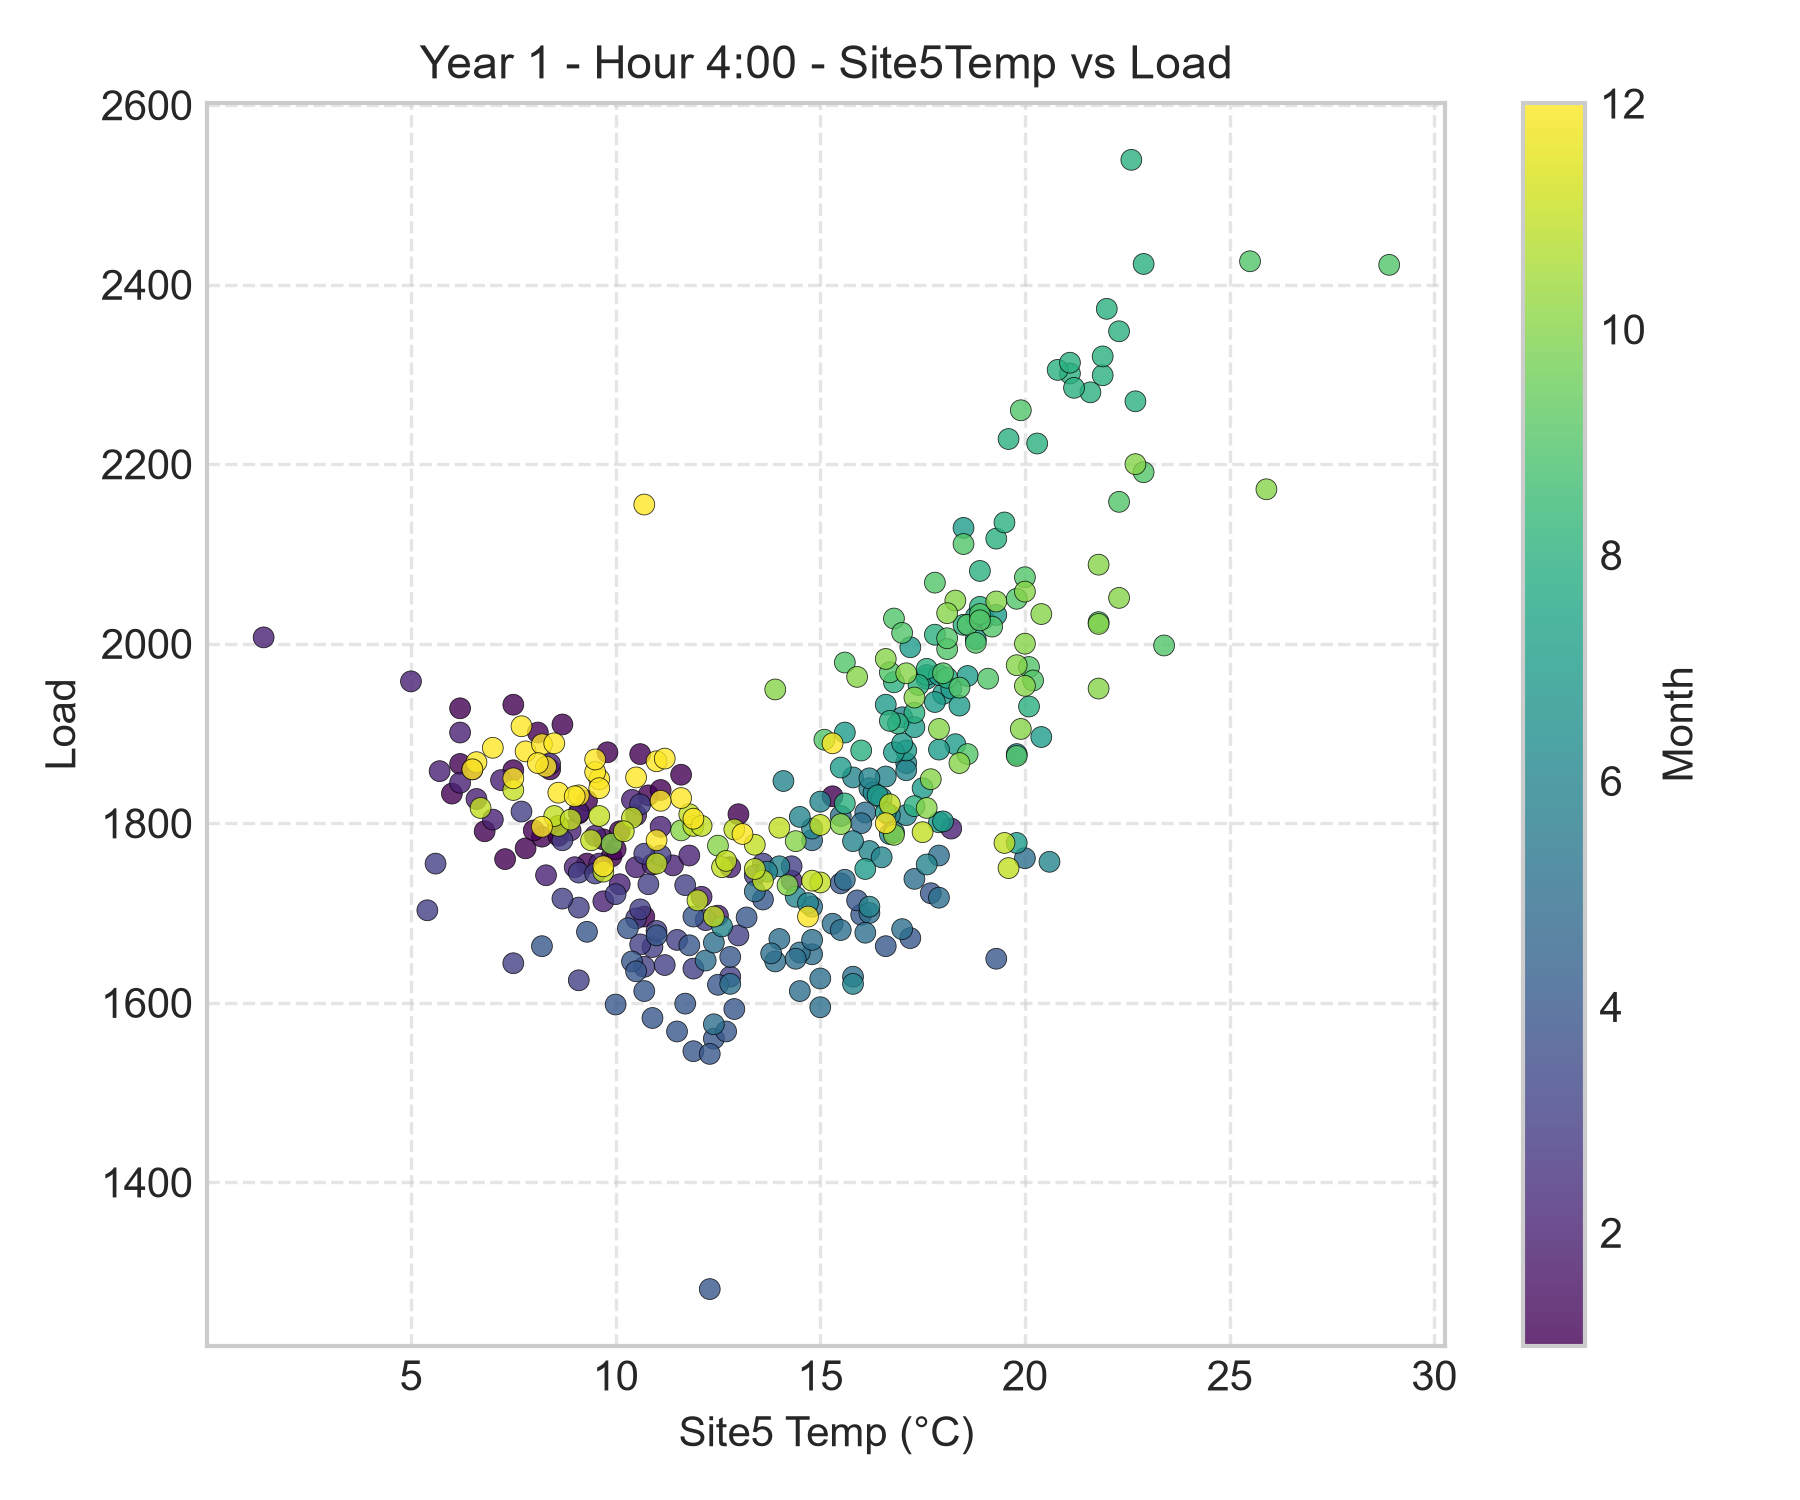
\includegraphics[width=\textwidth]{figures/Figure_1_Load_vs_Site5Temp_Year1.png}
        \caption{Năm thứ nhất (2020)}
    \end{subfigure}
    \hfill
    \begin{subfigure}[b]{0.48\textwidth}
        \centering
        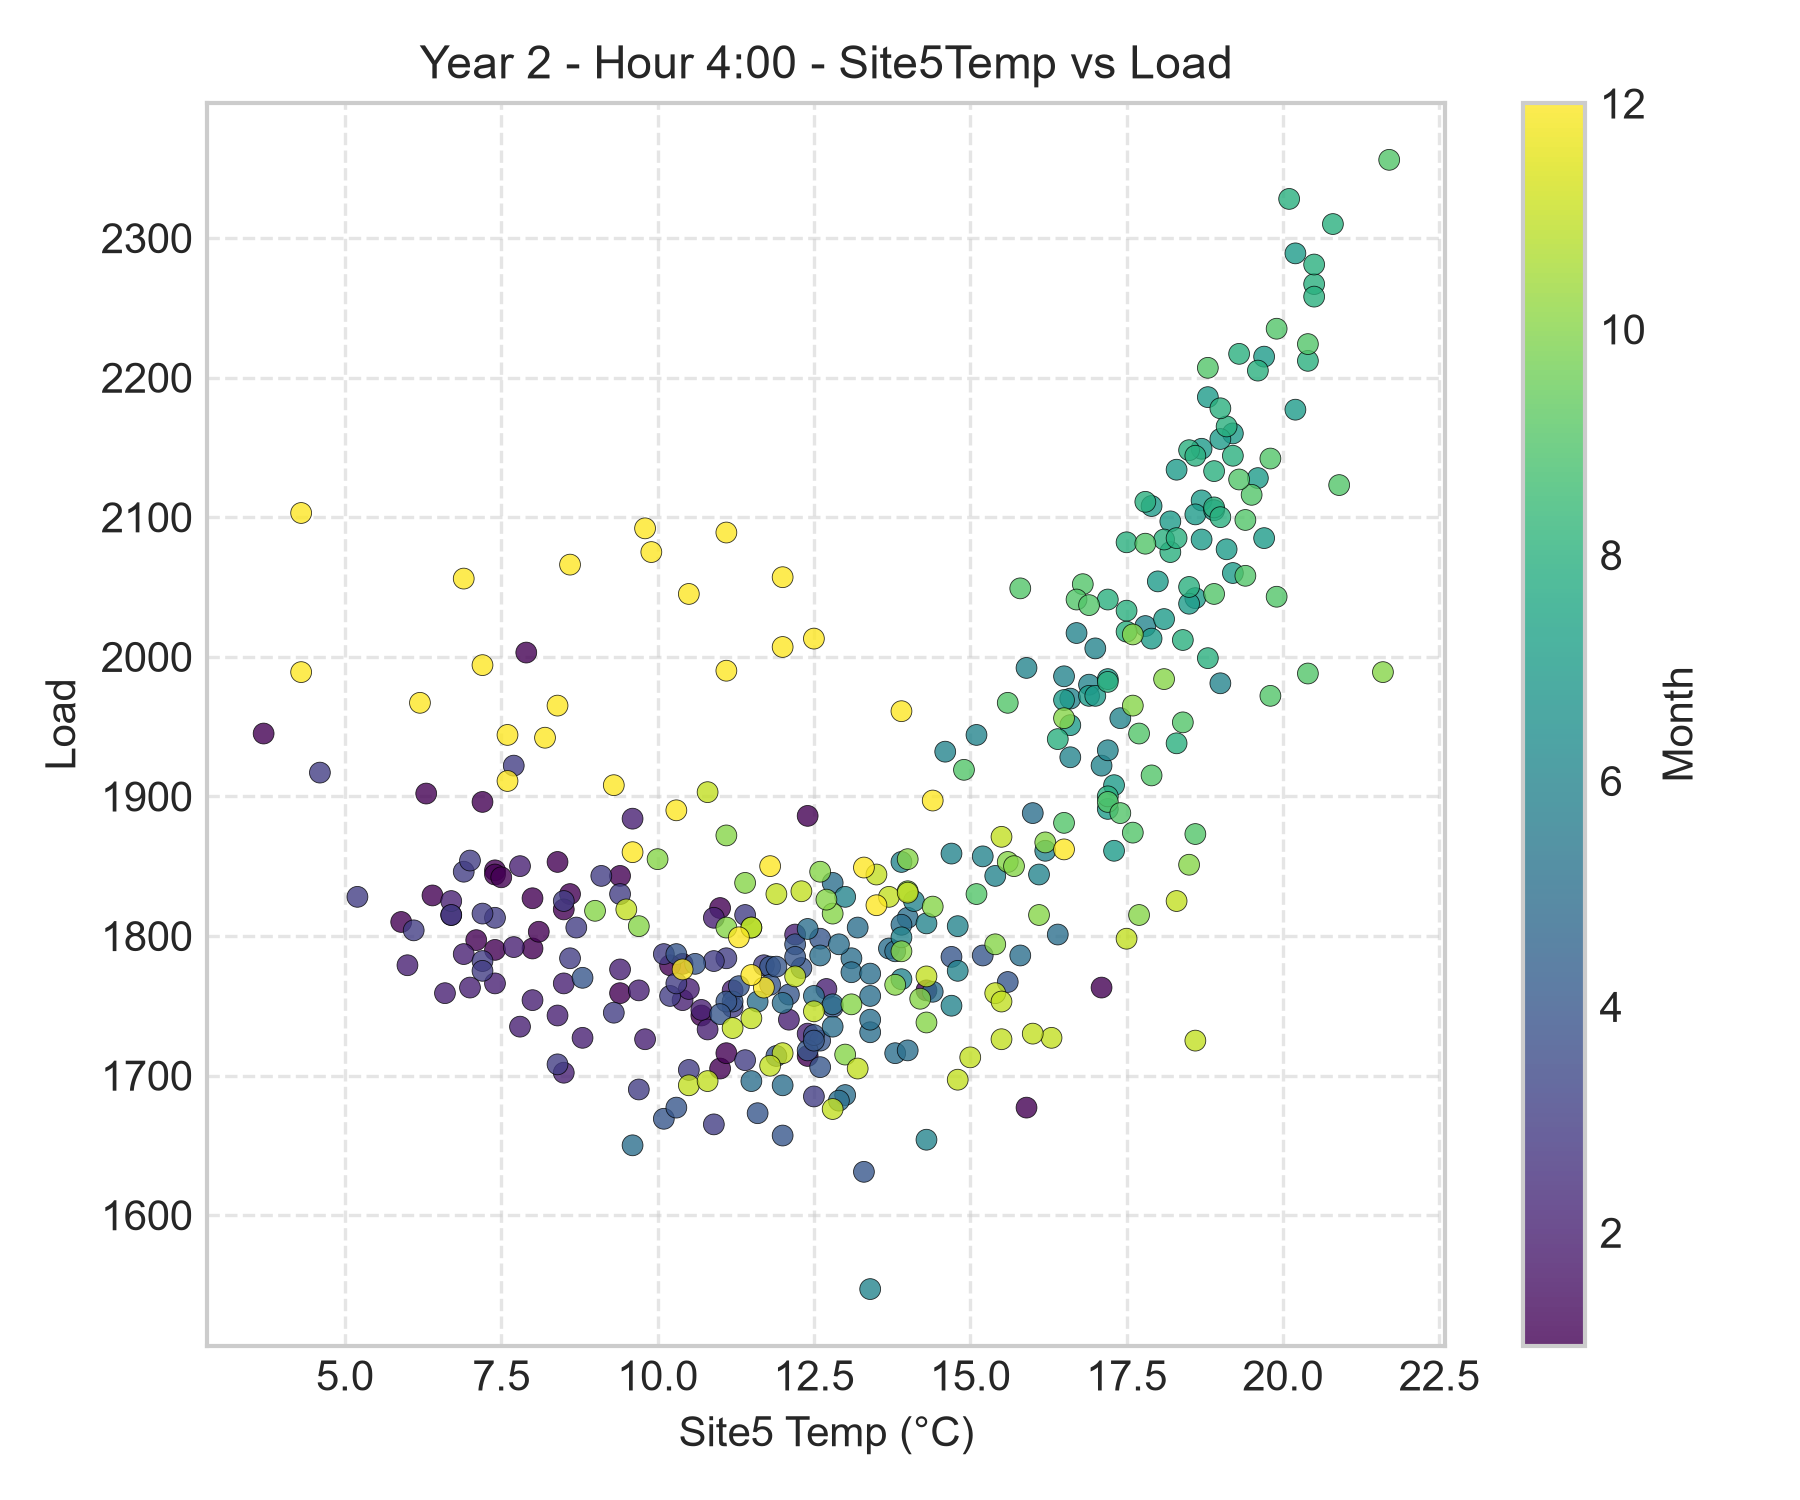
\includegraphics[width=\textwidth]{figures/Figure_2_Load_vs_Site5Temp_Year2.png}
        \caption{Năm thứ hai (2021)}
    \end{subfigure}
    \caption{Tương quan phi tuyến tính chữ U giữa phụ tải điện và nhiệt độ tại Trạm 5.}
    \label{fig:eda_temp_load}
\end{figure}

Hình~\ref{fig:eda_temp_load} thể hiện đồ thị phân tán giữa phụ tải điện và nhiệt độ tại Trạm 5. Đường cong tương quan biểu hiện dạng chữ U sắc nét: phụ tải đạt mức tối thiểu tại khoảng nhiệt độ tiện nghi $17^\circ\text{C}$--$19^\circ\text{C}$, và tăng phi tuyến tính rất dốc khi nhiệt độ vượt quá $25^\circ\text{C}$, minh chứng xác thực cho sự cần thiết của các đặc trưng ngưỡng vật lý HDD và CDD. Ngoài ra, sự khác biệt về mẫu hình phụ tải giữa ngày làm việc và ngày cuối tuần được thể hiện rõ nét trong Hình~\ref{fig:eda_weekdays}, cho thấy phụ tải công nghiệp và thương mại giảm mạnh vào thứ Bảy và Chủ Nhật.

\begin{figure}[htbp]
    \centering
    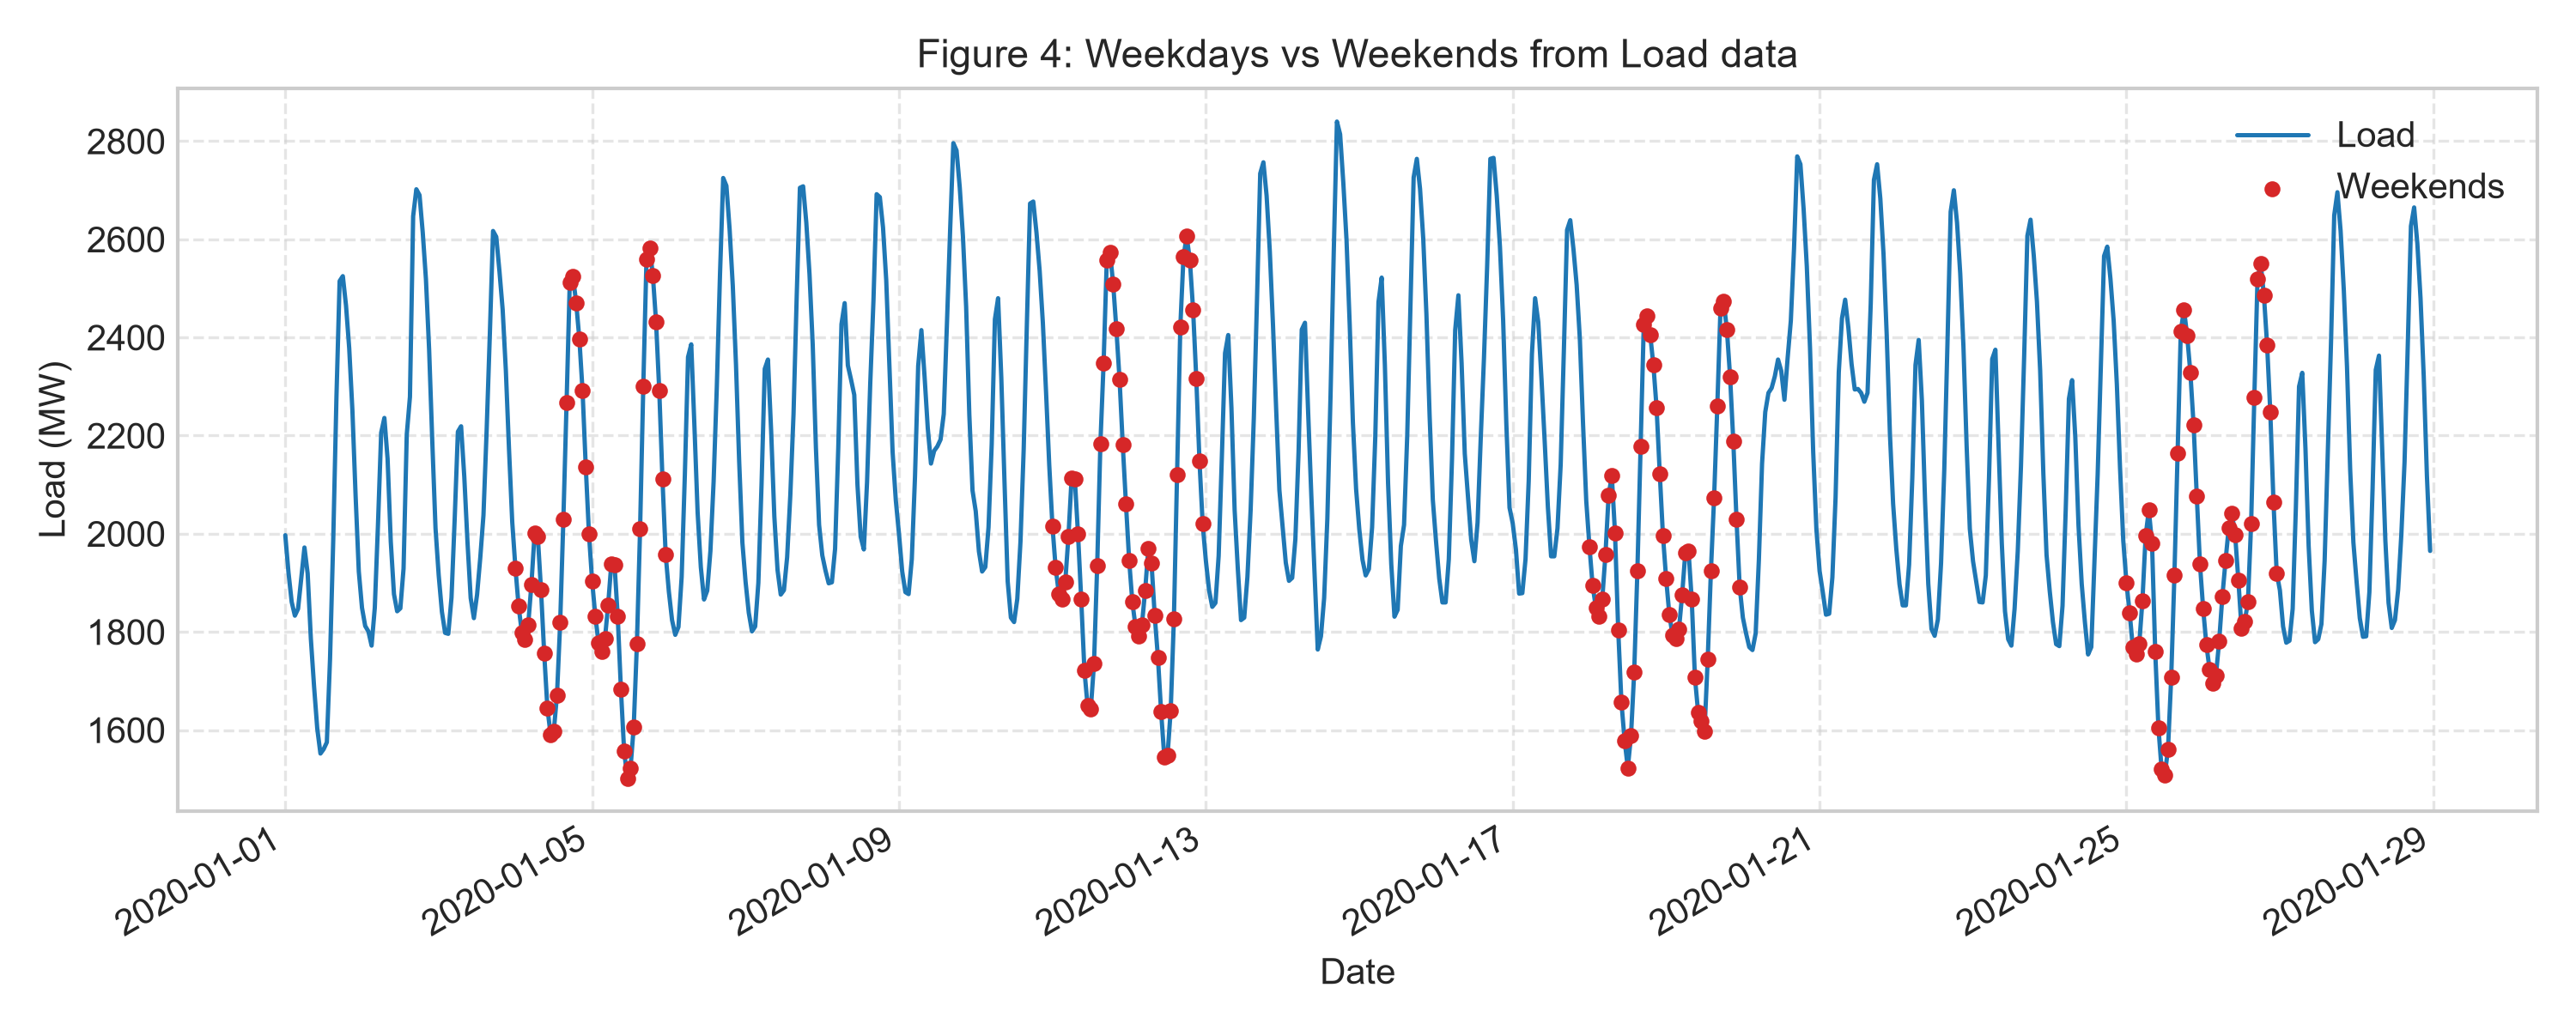
\includegraphics[width=0.75\textwidth]{figures/Figure_4_Weekdays_vs_Weekends.png}
    \caption{Phân phối đồ thị phụ tải giờ giữa Ngày làm việc và Ngày cuối tuần / Nghỉ lễ.}
    \label{fig:eda_weekdays}
\end{figure}

\subsection{Chiến lược Chia tập Dữ liệu (Data Splitting Protocols)}
Nhằm đảm bảo tính trung thực học thuật và ngăn chặn tuyệt đối hiện tượng rò rỉ dữ liệu xuyên thời gian (\textit{temporal data leakage}), mọi phép biến đổi đặc trưng (bao gồm việc fit các ma trận chiếu PCA, tính giá trị trung bình hay độ lệch chuẩn) đều chỉ được thực hiện nghiêm ngặt trên tập dữ liệu huấn luyện, sau đó áp dụng phép chiếu sang tập kiểm tra. Nghiên cứu triển khai bốn giao thức đánh giá chuẩn hóa:

\begin{enumerate}
    \item \textbf{Giao thức 1 (Year 1 $\to$ Year 2 Walk-Forward):} Huấn luyện toàn bộ pipeline trên dữ liệu Năm 1 (2020) và đánh giá khả năng ngoại suy trên toàn bộ dữ liệu Năm 2 (2021).
    \item \textbf{Giao thức 2 (Year 2 $\to$ Year 1 Generalization):} Huấn luyện trên dữ liệu Năm 2 (2021) và đánh giá trên dữ liệu Năm 1 (2020) nhằm kiểm tra tính đối xứng và độ nhạy của mô hình trước các biến động phân phối theo năm.
    \item \textbf{Giao thức 3 (5-Fold Time-Series Cross-Validation):} Chia liên tiếp tập dữ liệu 2 năm (17,544 giờ) thành 5 nếp gấp tịnh tiến thời gian theo cửa sổ mở rộng (\textit{expanding window}), không thực hiện xáo trộn ngẫu nhiên.
    \item \textbf{Giao thức 4 (Year 3 Unseen Test Benchmark):} Đây là thước đo đánh giá cao nhất của bài toán. Toàn bộ dữ liệu 2 năm đầu tiên (2020 và 2021) được dùng để huấn luyện mô hình, sau đó dự báo và đánh giá toàn diện trên 8,760 giờ độc lập của Năm thứ 3 (2022).
\end{enumerate}

\subsection{Thiết lập Huấn luyện và Không gian Siêu tham số}
Các mô hình được cấu hình và tối ưu hóa theo các tiêu chuẩn kỹ thuật sau:
\begin{itemize}
    \item \textbf{Kiến trúc 24-Hourly XGBoost:} Bao gồm 24 mô hình \texttt{XGBRegressor} hoạt động song song độc lập. Mỗi mô hình nhận các điểm dữ liệu thuộc đúng giờ $h \in \{1, \dots, 24\}$. Cấu hình chuẩn gồm $200$ cây quyết định, độ sâu tối đa $\text{max\_depth} = 6$, tốc độ học $\eta = 0.05$, hệ số tỷ lệ lấy mẫu con $\text{subsample} = 0.8$, và hàm mục tiêu hồi quy bình phương tối thiểu (\texttt{reg:squarederror}).
    \item \textbf{Mô hình Tuyến tính ElasticNet:} Được cấu hình với hệ số phạt chuẩn hóa $\alpha = 0.1$, tỷ lệ điều hòa hỗn hợp $\text{l1\_ratio} = 0.5$ (chia đều trọng số giữa chuẩn $L_1$ và chuẩn $L_2$), số vòng lặp tối đa $2,000$ và hạt giống ngẫu nhiên $\text{random\_state} = 42$.
    \item \textbf{Mô hình Meta-Learner (LightGBM):} Nhận vector đầu vào gồm dự báo OOF của ElasticNet, XGBoost cùng vector ngữ cảnh thời gian - khí tượng thực. Siêu tham số được tinh chỉnh tự động qua 15 vòng lặp thử nghiệm của Optuna trên 3 nếp gấp TimeSeriesSplit với không gian tìm kiếm: $\text{n\_estimators} \in [50, 250]$, $\text{max\_depth} \in [2, 6]$, $\text{learning\_rate} \in [0.01, 0.2]$, $\text{num\_leaves} \in [7, 31]$, $\text{reg\_alpha} \in [10^{-3}, 5.0]$, $\text{reg\_lambda} \in [0.1, 10.0]$.
\end{itemize}

Thí nghiệm được triển khai trên môi trường Python 3.10 với các thư viện mã nguồn mở: \texttt{xgboost 2.0.3}, \texttt{lightgbm 4.3.0}, \texttt{scikit-learn 1.4.1}, \texttt{optuna 3.5.0}, \texttt{shap 0.44.1}. Nhờ cơ chế tính toán phân tán đa luồng (\texttt{n\_jobs=-1}), toàn bộ pipeline từ tiền xử lý, huấn luyện 24 mô hình con, tối ưu hóa meta-learner cho tới kết xuất đồ thị hoàn tất trong vòng dưới 3 phút trên máy trạm thông thường.

\subsection{Thiết lập Đánh giá}
Kết quả dự báo được tính toán theo 5 chỉ số: RMSE, MAE, MAPE, sMAPE và $R^2$. Tất cả các thí nghiệm so sánh đều được cố định hạt giống ngẫu nhiên (\textit{random seed} $= 42$) để đảm bảo $100\%$ tính tái lập thực nghiệm. Kết quả của mô hình đề xuất được đối chiếu trực tiếp với các số liệu công bố trong bài báo gốc của Roy et al.~\cite{roy2025hourly} cũng như các mô hình đơn lẻ độc lập.
